\documentclass{article}
\usepackage{amsmath}
\usepackage{amssymb}
\usepackage{amsbsy}
\usepackage{bbm}
\usepackage{url}
\usepackage{color}
\usepackage{float}
\usepackage{graphicx}
\usepackage{epstopdf}
\usepackage{fancyhdr}
\usepackage{enumerate}
\usepackage{tikz}
\usepackage[ruled,vlined]{algorithm2e}
\usepackage[colorlinks=true,urlcolor=blue]{hyperref}
\usepackage[utf8]{inputenc}
\newcommand{\Solution}[1]{{\medskip \color{red} \bf $\bigstar$~\sf \textbf{Solution}~$\bigstar$ \sf #1 } \bigskip}
\title{Machine Learning with Graphs\\
Homework 1}


\begin{document}

\maketitle



\section*{1 Node Embedding and its Relation to Matrix Factorization}

What to submit: For Q2.1, one or more sentences/equations describing the decoder. For Q2.2, write down the objective function. For Q2.3, describe the characteristics of $W$ in one or more sentences. For Q2.4, write down the objective function. For Q2.5, characterize the embeddings, whether you think it will reflect structural similarity, and your justification. For Q2.6, one or more sentences for node2vec and struct2vec respectively. For Q2.7, one or more sentences of explanation. For Q2.8, one or more sentences characterizing embeddings from struct2vec.
\\

Recall that matrix factorization and the encoder-decoder view of node embeddings are closely related. For the embeddings, when properly formulating the encoder-decoder and the objective function, we can find equivalent matrix factorization formulation approaches.

Note that in matrix factorization we are optimizing for L2 distance; in encoder-decoder examples such as DeepWalk and node2vec, we often use log-likelihood as in lecture slides. The goal to approximate $A$ with $Z^TZ$ is the same, but for this question, stick with the L2 objective function.

\subsection*{2.1 Simple matrix factorization}

In the simple matrix factorization, the objective is to approximate adjacency matrix $A$ by the product of embedding matrix with its transpose. The optimization objective is $\min_Z \|A - Z^TZ\|^2$.

In the encoder-decoder perspective of node embeddings, what is the decoder? (Please provide a mathematical expression for the decoder)

\Solution{The Decoder will be: $\mathbf{{f}_decoder(z_i,z_j)}=z_i^Tz_j$  or, for decoding the entire graph: $Z^tZ$\}

\subsection*{1.2 Alternate matrix factorization}

In linear algebra, we define bilinear form as $z_i^T W z_j$, where $W$ is a matrix. Suppose that we define the decoder as the bilinear form, what would be the objective function for the corresponding matrix factorization? (Assume that the $W$ matrix is fixed)

\Solution{We should minimize $\mathbf{min_Z}\|A-Z^T WZ\|^2$

\subsection*{2.3 BONUS: Relation to eigen-decomposition}

Recall eigen-decomposition of a matrix. What would be the condition of $W$, such that the matrix factorization in the previous question (2.2) is equivalent to learning the eigen-decomposition of matrix $A$?

\Solution{Since we know ${A∈\{\mathbb R^{n\times n} ∣A ^⊤ =A\}} $  we know that $A=U^TDU$, where ${D=diag(\lambda_1,\lambda_2,...,\lambda_n)}$ so we can enforce on W the condition that $W=D$ to get the wanted result, meaning learning $Z$ is actually learning the unitary matrix $U$.

\subsection*{2.4 Multi-hop node similarity}

Define node similarity with the multi-hop definition: 2 nodes are similar if they are connected by at least one path of length at most $k$, where $k$ is a parameter (e.g. $k = 2$). Suppose that we use the same encoder (embedding lookup) and decoder (inner product) as before. What would be the corresponding matrix factorization problem we want to solve?

\Solution{}

\subsection*{1.5 node2vec \& struct2vec (i)}

Finally, we’ll explore some limitations of node2vec that are introduced in the lecture, and look at algorithms that try to overcome them.

As mentioned in the lecture, due to the way random walk works, it’s hard for node2vec to learn structural embedding from the graph. Think about how a new algorithm called struct2vec works. For this question, we define a clique to be a fully connected graph, where any two nodes are connected.

Given a graph $G(V,E)$, it defines $K$ functions $g_k(u, v)$, $k = 1, 2, .., K$, which measure the structural similarity between nodes. The parameter $k$ means that only the local structures within distance $k$ of the node are taken into account. With all the nodes in $G$, regardless of the existing edges, it forms a new clique graph where any two nodes are connected by an edge whose weight is equal to the structural similarity between them. Since struct2vec defines $K$ structural similarity functions, each edge has a set of possible weights corresponding to $g_1, g_2, ..., g_K$.

The random walks are then performed on the clique. During each step, weights are assigned according to different $g_k$’s selected by some rule (omitted here for simplification). Then, the algorithm chooses the next node with probability proportional to the edge weights.

Characterize the vector representations (i.e. the embedding space) of the 10-node cliques after running the node2vec algorithm on the graph in figure \ref{fig:10-node-cliques}. Assume through the random walk, nodes that are close to each other have similar embeddings. Do you think the node embeddings will reflect the structural similarity? Justify your answer.

\begin{figure}[h]
\centering
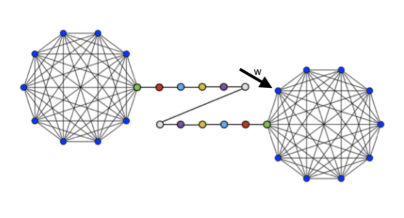
\includegraphics[width=0.5\textwidth]{10_node_cliques.png}
\caption{Two 10-node cliques}
\label{fig:10-node-cliques}
\end{figure}


\Solution{}

\subsection*{1.6 node2vec \& struct2vec (ii)}

In the above figure \ref{fig:10-node-cliques}, suppose you arrive at node $w$. What are the nodes that you can reach after taking one step further with the node2vec algorithm? What about with the struct2vec algorithm (suppose that for this graph, $g_k(u, v) > 0$ for any $u,v,k$)?

\Solution{}

\subsection*{1.7 node2vec \& struct2vec (iii)}

Why is it necessary to consider different $g_k$’s during the random walk?

\Solution{}

\subsection*{1.8 node2vec \& struct2vec (iv)}

Characterize the vector representations (i.e. the embedding space) of the two 10-node cliques after running the struct2vec algorithm on the graph in the above figure (\ref{fig:10-node-cliques}).

\Solution{}

\end{document}